\documentclass[preprint,12pt]{elsarticle}

\usepackage[utf8]{inputenc}
\usepackage[T1]{fontenc}
\usepackage{amsmath,amssymb,amsfonts}
\usepackage{graphicx}
\usepackage{booktabs}
\usepackage{tabularx}
\usepackage{array}
\usepackage{enumitem}
\usepackage[hidelinks]{hyperref}

\newcolumntype{Y}{>{\raggedright\arraybackslash}X}
\newcolumntype{C}{>{\centering\arraybackslash}X}
\graphicspath{{../figures_v2/}}
\emergencystretch=2em

\journal{Robotics and Autonomous Systems}

\begin{document}

\begin{frontmatter}

\title{RoboTeach: Structured Task Grounding, Multi-View Perception, and Feedback-Driven Calibration for Language-Guided Robotic Manipulation}

\author[omu]{Muhammed Emin \c{C}elik}
\ead{muhammedemin.celik@omu.edu.tr}
\author[omu]{Bar\i\c{s} Kaya}
\ead{baris.kaya@omu.edu.tr}
\author[omu]{Mahmut \"{O}zt\"{u}rk}
\ead{mahmut.ozturk@omu.edu.tr}
\author[omu]{\.{I}smail \.{I}\c{s}eri\corref{cor1}}
\ead{ismail.iseri@omu.edu.tr}

\cortext[cor1]{Corresponding author.}
\address[omu]{Department of Computer Engineering, Ondokuz May\i s University, Samsun, T\"{u}rkiye}

\begin{abstract}
Converting natural language commands into reliable robot motions is difficult when the scene is only partially visible and contact with objects depends on friction. This paper presents RoboTeach, a training-free system that generates robot code with a large language model (LLM). The system assigns Turkish and English commands to one of six task types with a rule-based parser, estimates object positions from four cameras, checks the generated code before execution, and updates the motion settings of each task type using feedback from a vision-language model after every iteration. The system was tested with a Franka Emika Panda arm in PyBullet simulation on six tabletop tasks, with 30 random initial scenes per task. RoboTeach completed 157 of 180 trials (87.2\%), whereas an open-loop baseline using the same four cameras succeeded in 106 trials (58.9\%). When physics and sensor parameters were randomized, these rates were 81.7\% and 54.4\%, respectively. The parser assigned all 180 command phrasings to the correct task type. Ablation experiments show that most of the gain comes from task parsing and multi-camera perception. Saved calibration settings gave no additional gain while automatic safe lifting was enabled (154/180 vs.\ 159/180, $p = 0.332$). With safe lifting disabled, calibration raised success from 80.0\% to 82.8\%, but the difference was not statistically significant ($p = 0.442$).
\end{abstract}

\begin{keyword}
Robotic manipulation \sep Large language models \sep Feedback-driven calibration \sep Multi-view perception \sep Vision-language critics \sep Robot simulation
\end{keyword}

\end{frontmatter}

\section{Introduction}

Converting natural language commands into reliable physical motions in tabletop manipulation is not yet a solved problem~\cite{billard2019trends,kroemer2021review}. The difficulty arises because cameras see the scene only partially and contact with objects depends on friction. Integrated task and motion planning (TAMP) approaches can produce geometrically feasible plans when object models are complete and domain knowledge is defined by hand~\cite{garrett2021tamp}. These approaches become less flexible, however, when a free-form user command must be matched to noisy scene observations on the fly. Pretrained language and multimodal models have considerably reduced the effort of writing rules by hand. Work in this direction includes affordance scoring~\cite{ahn2022saycan}, code generation with Code-as-Policies~\cite{liang2023cap,singh2023progprompt}, three-dimensional value maps~\cite{huang2023voxposer}, and vision-language-action (VLA) policies that map images directly to actions, such as OpenVLA~\cite{kim2024openvla}, Octo~\cite{ghosh2024octo}, and $\pi_0$~\cite{black2025pi0}.

Training-free language-based manipulation systems face three types of failure once simulation shortcuts such as artificial grasp constraints and object teleportation are removed. First, open-loop code policies estimate object positions only from the depth image of an overhead camera. Because this image measures only the top surface, the position of a lower block in a stack is computed incorrectly. A low default transit height also causes the robot to strike obstacles or towers that have already been built. Second, closed-loop methods such as inner monologue~\cite{huang2022inner}, experience summarization~\cite{liu2023reflect}, verbal reinforcement~\cite{shinn2023reflexion}, and iterative self-refinement~\cite{madaan2023selfrefine} append correction suggestions extracted from failed trials to the input of the language model as plain text. Because language models can overlook information in the middle of long inputs~\cite{liu2024lost}, these suggestions do not change motion parameters directly and can degrade position calculations. Third, when correction suggestions are saved under task names that the language model generates itself each time, a saved suggestion is not found if the same task is requested with different words.

Neuro-symbolic and agentic robot architectures aim to remove these shortcomings by combining the flexibility of language models with explicitly defined task representations~\cite{marra2024neurosymbolic,frering2025bdi,zhao2026agentic}. RoboTeach is not a new foundation model. It is a training-free system that combines an existing LLM with rule-based task parsing, multi-camera perception, code checking, and feedback-driven calibration. The contributions of this work are as follows:
\begin{itemize}[leftmargin=*]
\item a rule-based task parser that assigns Turkish and English commands to one of six task types and gives the language model a placement instruction for each task type;
\item a four-camera perception method that estimates the position of covered blocks from side cameras;
\item a calibration loop that updates motion settings per task type and is checked separately against ground-truth positions read from the simulator;
\item experiments that measure the contribution of each component and the conditions under which calibration is needed.
\end{itemize}

\section{Related Work}

\subsection{Task and Motion Planning, Code Generation, and Generalist Policies}

Hierarchical TAMP solvers combine discrete symbolic operators with continuous geometric samplers~\cite{kaelbling2011hpn,garrett2020pddlstream}. These approaches, however, require domain knowledge to be written by an expert in the Planning Domain Definition Language (PDDL). Large language models reduce this dependency. Text2Motion~\cite{lin2023text2motion} produces feasible plans from natural language commands, and TidyBot~\cite{wu2023tidybot} generalizes a user's placement preferences from a few examples. ReKep~\cite{huang2024rekep} optimizes relational keypoint constraints produced by a vision-language model over trajectories that jointly describe the position and orientation of the gripper. Generalist multimodal policies follow a different path. Models such as PaLM-E~\cite{driess2023palme}, RT-2~\cite{zitkovich2023rt2}, TinyVLA~\cite{wen2025tinyvla}, $\pi_0$~\cite{black2025pi0}, and OpenVLA-OFT~\cite{kim2025openvlaoft} learn to map images directly to actions from large-scale real-world demonstration data. Unlike these policies, RoboTeach requires neither demonstration data nor fine-tuning. The system builds on Code-as-Policies~\cite{liang2023cap} and ProgPrompt~\cite{singh2023progprompt} and extends them with code checking, frictional contact physics, and calibration records kept per task type.

\subsection{Multi-View Perception, Grasping, and Motion Control}

PerAct~\cite{shridhar2023peract} processes language commands and three-dimensional voxel observations with a transformer network to produce manipulation actions. Diffusion Policy~\cite{chi2024diffusion} generates robot actions through a diffusion process and can learn more than one valid way of moving for the same task. Vision-language features~\cite{radford2021clip} allow objects to be recognized without task-specific training, and point cloud processing methods~\cite{rusu2011pcl} allow three-dimensional geometry to be extracted. However, a depth image from a single overhead camera systematically misestimates the position of tall objects and covered blocks. Reliable grasping with a parallel-jaw gripper requires friction and force-closure conditions to be satisfied at the contact points~\cite{bicchi2000grasping}. Analytical and data-driven methods have been developed for selecting suitable grasp points~\cite{bohg2014grasp}. To avoid sudden accelerations, motions are smoothed with fifth-order minimum-jerk profiles~\cite{flash1985coordination}. This study uses the Franka Emika Panda arm~\cite{haddadin2022franka}. Randomly varying simulation parameters, known as domain randomization~\cite{tobin2017domain}, is used to test the robustness of systems developed in simulation.

\subsection{Vision-Language Critics and Feedback-Driven Calibration}

Voyager~\cite{wang2024voyager}, Eureka~\cite{ma2024eureka}, and work that uses vision-language models as reward functions~\cite{rocamonde2024vlmrm} iteratively update robot code or reward functions according to outcomes from the environment. AHA~\cite{duan2025aha} developed a vision-language critic that detects and explains manipulation failures. ReflectVLM~\cite{feng2025reflectvlm} uses a reflection step based on visual foresight in multi-stage planning. Zhao et al.~\cite{zhao2026agentic} combined LLM task proposals with vision-language verification for skill discovery. On the other hand, studies of language models used as judges~\cite{zheng2023judging} have shown that relying on a judge from the same model family, or on unverified textual assessments, can hide systematic errors. For this reason, critic decisions were not used directly in this study; the decisions of two different critic models were compared with ground-truth object positions read from the simulator. Agreement was measured with Cohen's kappa~\cite{cohen1960kappa} and the Landis--Koch agreement bands~\cite{landis1977kappa}.

\section{Method}

\subsection{System Architecture}

RoboTeach converts a natural language command into robot motion in six steps (Fig.~\ref{fig:arch}). In the first step, a rule-based parser assigns the command to one of six task types and orders the objects mentioned in the command. In the second step, object positions in the scene are estimated from four color and depth (RGB-D) cameras. In the third step, an LLM is given the object positions, a placement instruction specific to the task type, and the current motion settings, and generates a short Python program. In the fourth step, the program is executed on the robot after it is checked to contain only permitted commands. In the fifth step, a vision-language model (VLM) looks at images of the scene from three cameras and decides whether the task succeeded. In the last step, if the iteration failed, the failure type is identified and the motion settings of that task type are updated together with a short correction rule. This calibration loop continues until two consecutive iterations are judged successful or five iterations are completed. In the evaluation trials run after calibration, success is determined from ground-truth object positions read from the simulator rather than from the VLM decision.

\begin{figure}[htbp]
\centering
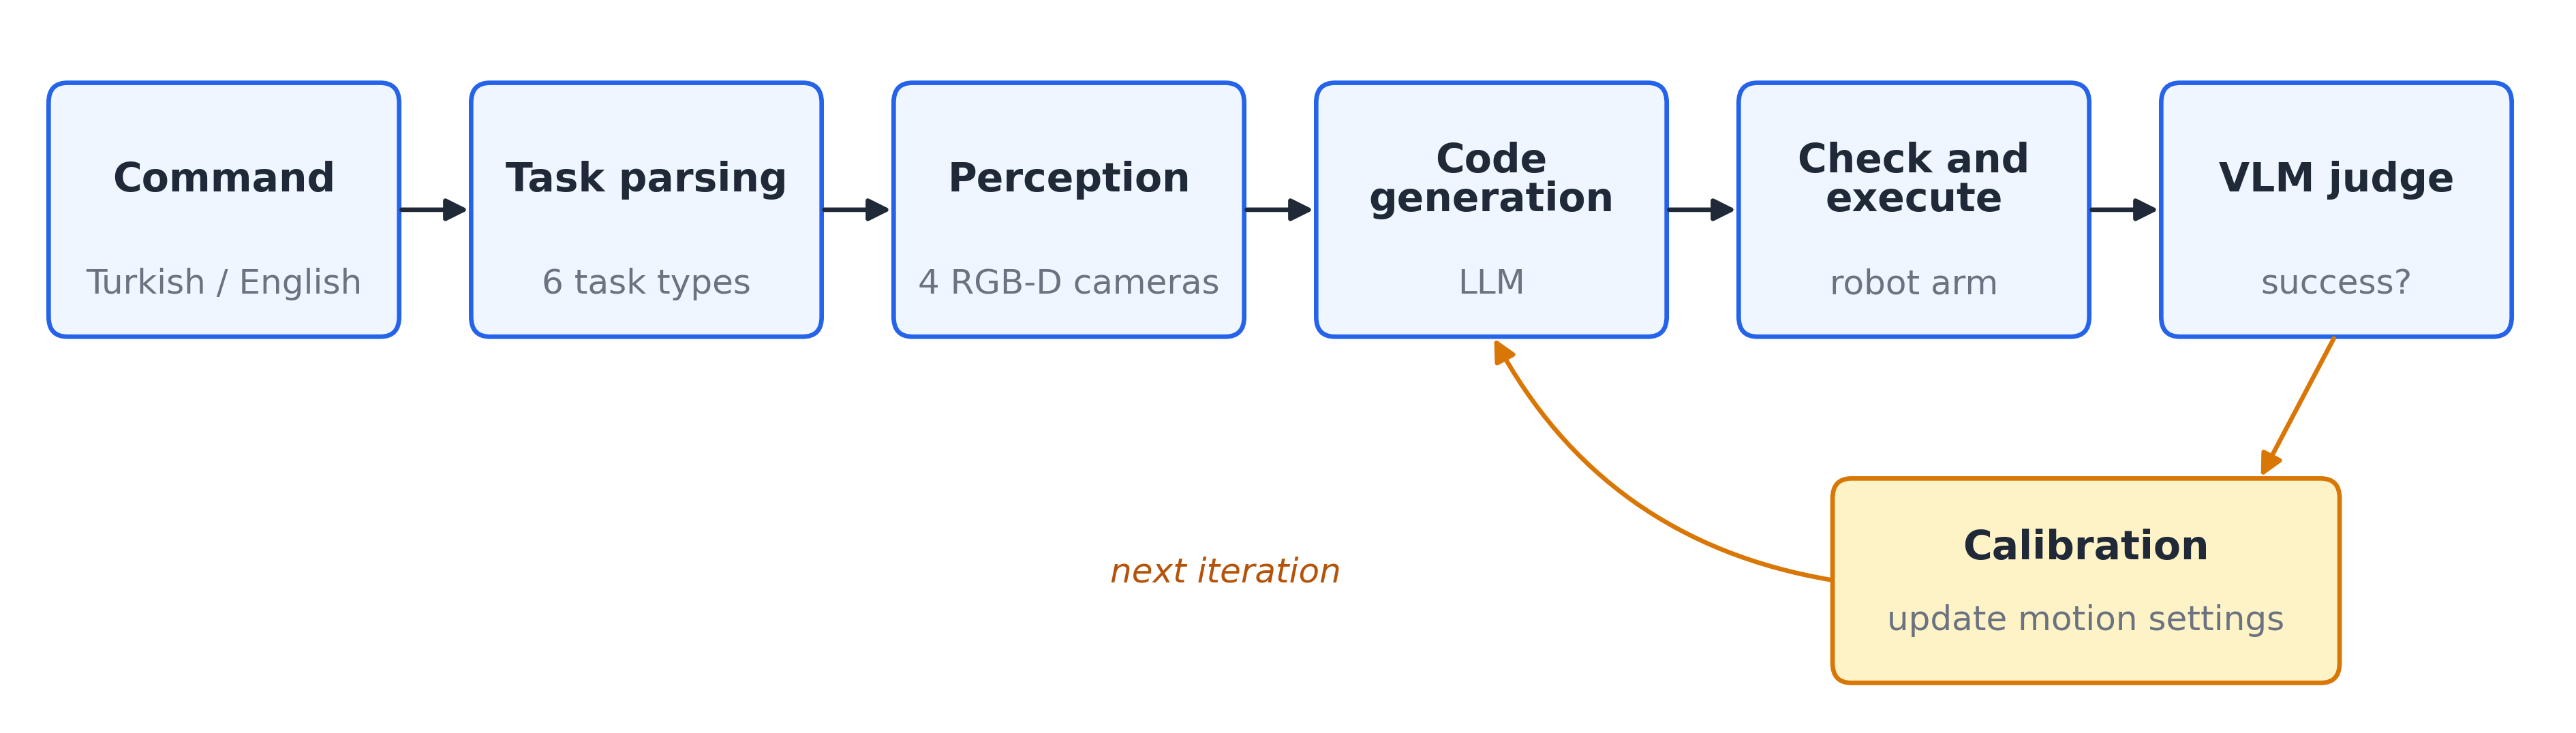
\includegraphics[width=\textwidth]{fig1_architecture.png}
\caption{System architecture.}
\label{fig:arch}
\end{figure}

\subsection{Simulation Environment and Tasks}

Experiments were run in the PyBullet physics engine at a step rate of 240~Hz. No artificial constraints attaching objects to the robot and no teleportation moving objects directly to their targets were used. A seven-joint Franka Emika Panda arm is mounted at the edge of a 1.10~m $\times$ 1.10~m table. The table holds four 50~mm cubes colored red, blue, green, and yellow, whose initial positions are randomized in every trial. The table also holds an open-top box (inner dimensions 13.8~cm $\times$ 13.8~cm, wall height 70~mm). In the Obstacle task, an 11~cm high wall is placed between the start and goal regions.

The system was tested on six tabletop tasks. The tasks, example commands, and success conditions are given in Table~\ref{tab:tasks}. Success is determined at the end of each trial from ground-truth object positions read from the simulator. A cube falling off the table counts as a failure regardless of the task type. Fig.~\ref{fig:tasks} shows the tasks in simulation.

\begin{table}[htbp]
\centering
\caption{Tasks, example commands, and success conditions.}
\label{tab:tasks}
\begin{tabularx}{\textwidth}{@{}l Y Y@{}}
\toprule
Task & Example command & Success condition \\
\midrule
Tower & ``Stack the blocks like a tower: blue at the bottom, red on it, green on it, and yellow on top'' & The four cubes stand on top of each other in the given order. \\
Row & ``Line up the red, blue, green, and yellow cubes side by side in a single row'' & The four cubes stand in a single row with gaps of 46--95~mm. \\
Diagonal & ``Put the blue block diagonal to the red one and the green block diagonal to the yellow one'' & The moved cube is offset by 35--115~mm from the reference cube along both axes. \\
Box & ``Put the red, blue, and green cubes inside the brown box'' & All three cubes are inside the box. \\
Swap & ``Put the blue cube on the red one, but the red one is already on the blue one'' & The blue cube is on top of the red cube. \\
Obstacle & ``Lift the blue cube over the obstacle and put it on the red cube'' & The blue cube is on top of the red cube. \\
\bottomrule
\end{tabularx}

\vspace{2pt}
\begin{minipage}{\textwidth}\small
\textit{Note:} In tasks that require stacking (Tower, Swap, Obstacle), each cube must be offset horizontally by at most 32~mm and tilted by at most 0.35~rad relative to the cube below it. In the Obstacle task, collisions between the robot and the wall are not checked; only the final state is evaluated.
\end{minipage}
\end{table}

\begin{figure}[htbp]
\centering
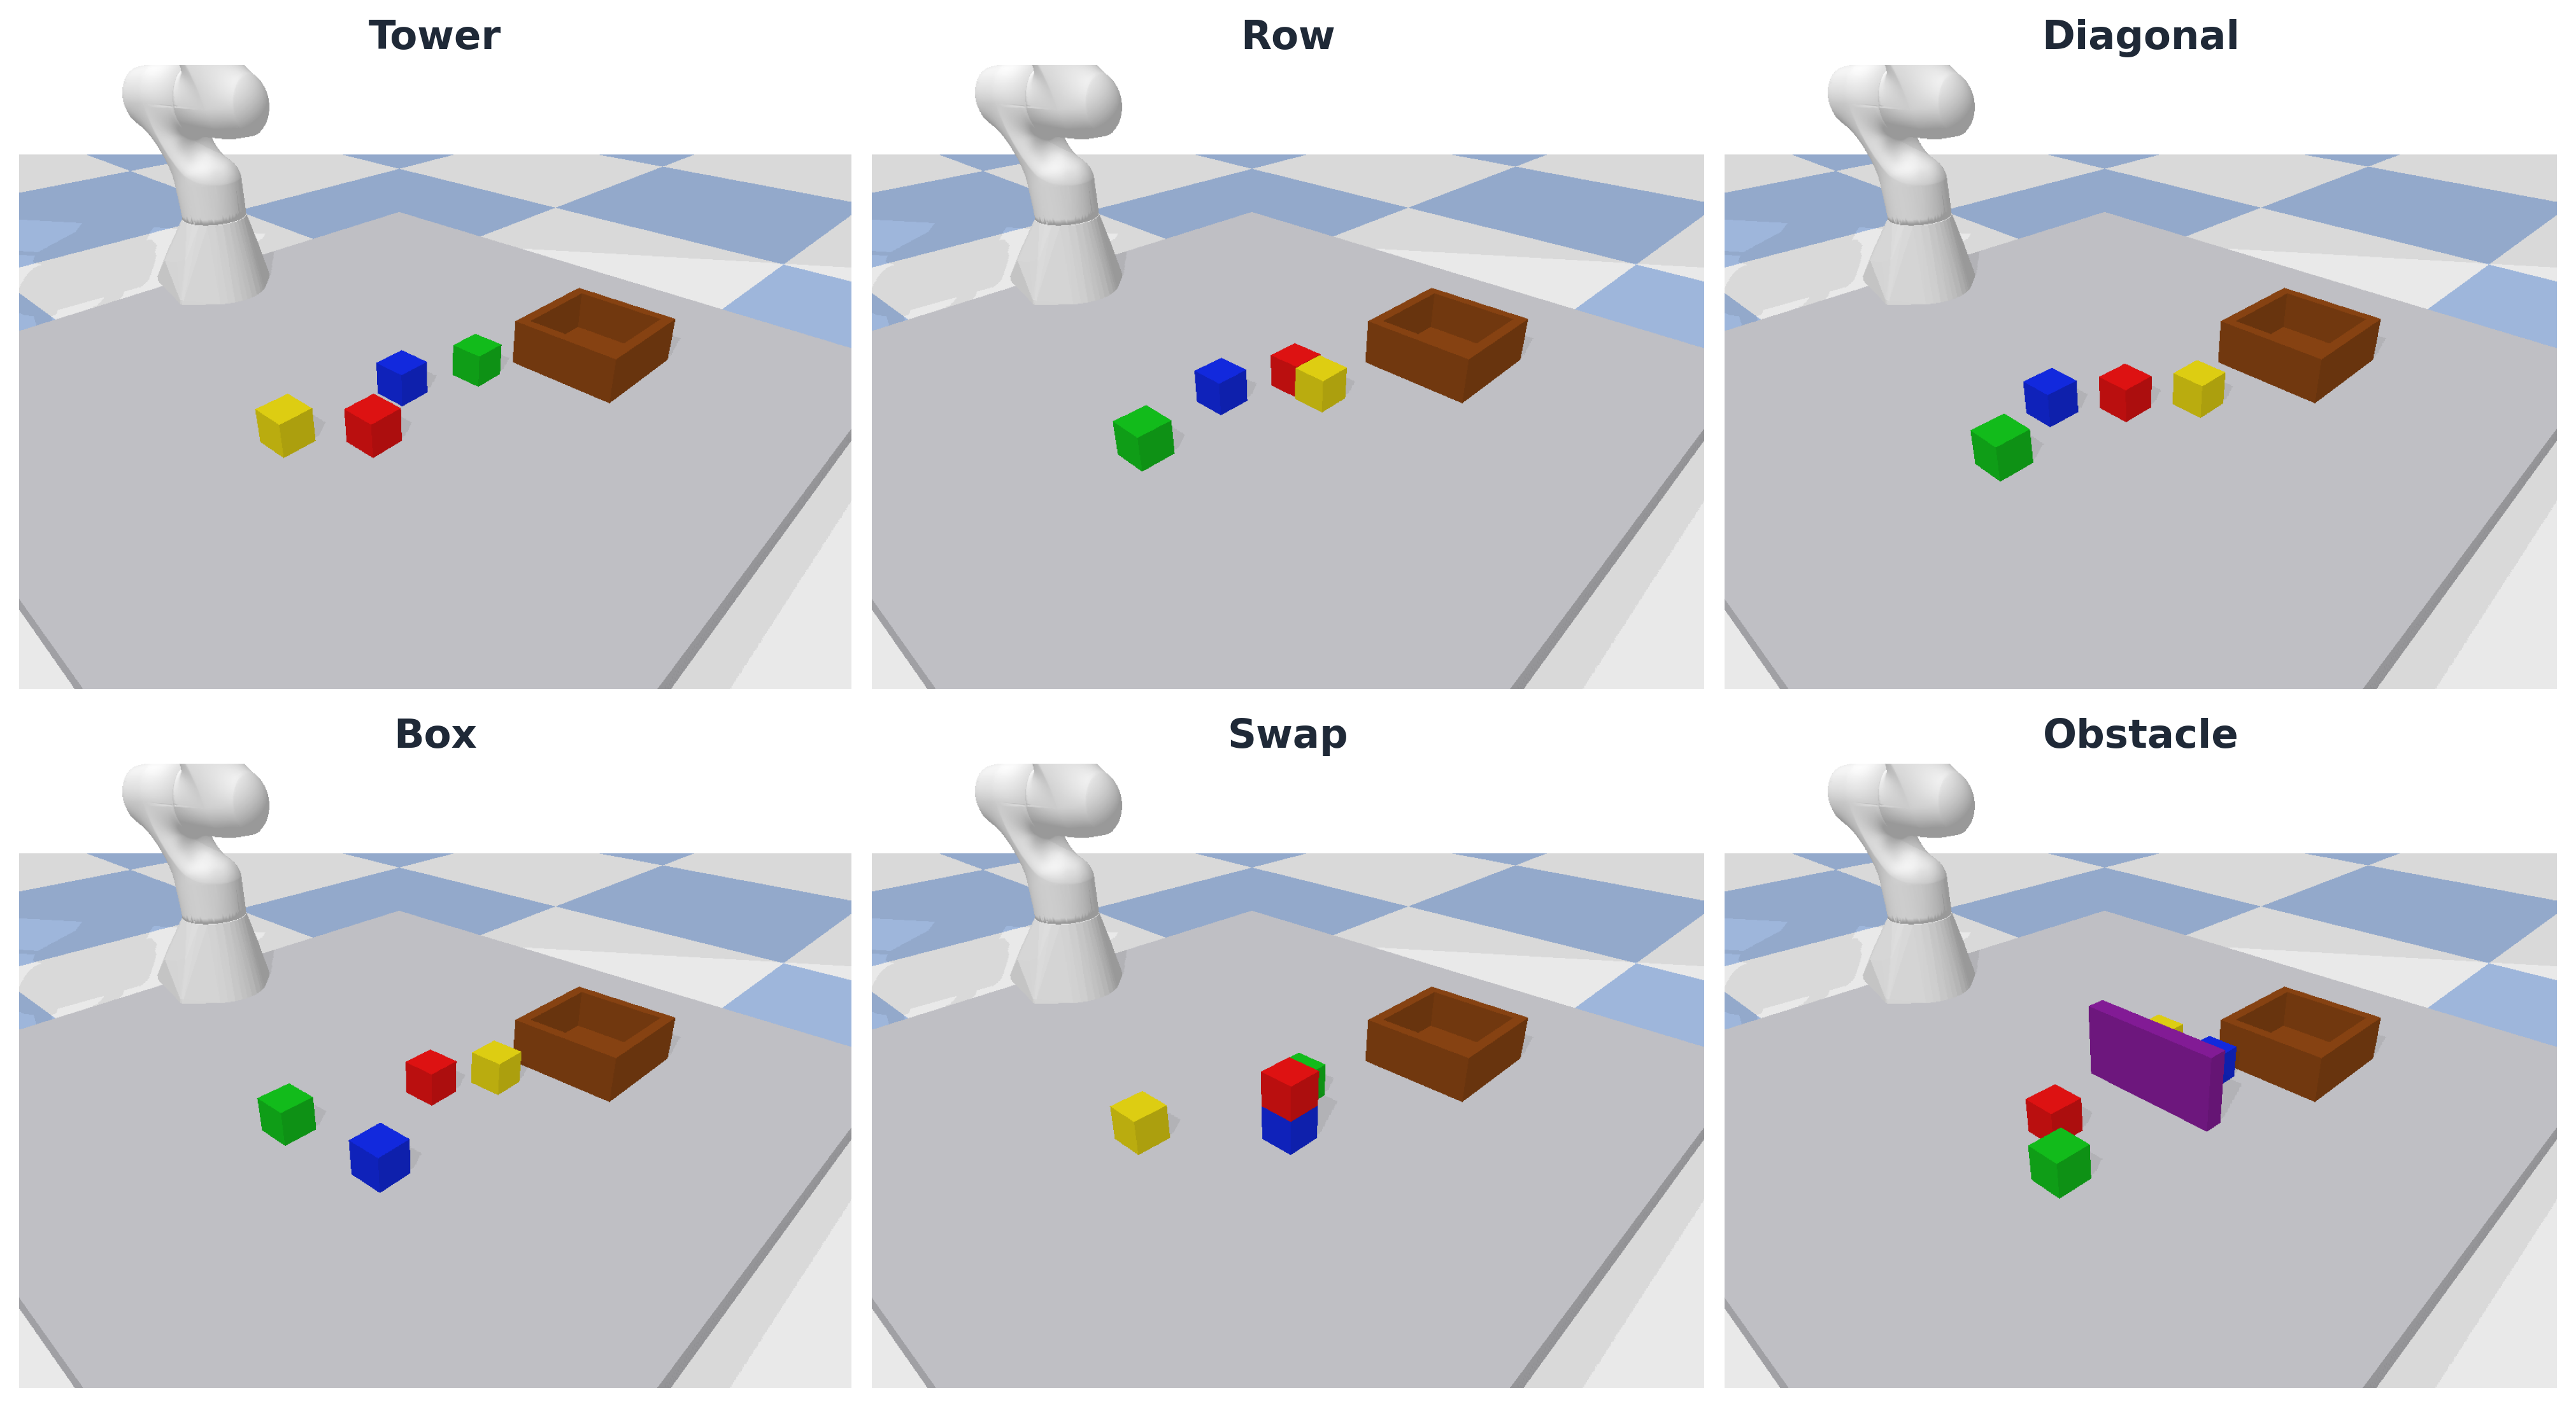
\includegraphics[width=\textwidth]{fig2_tasks.png}
\caption{Initial scenes of the tasks in simulation.}
\label{fig:tasks}
\end{figure}

\subsection{Task Parsing}

The parser is a rule-based program built on Turkish and English keywords and patterns. For example, the words ``\"{u}st \"{u}ste'', ``kule'', or ``stack'' route a command to a stacking task, ``yan yana'' or ``in a row'' route it to the Row task, and ``i\c{c}ine'' or ``inside'' route it to the Box task. In addition to assigning the command to one of six task types, the parser extracts the order of the objects, the pairs of moved and reference cubes, the target box, the cubes that are initially stacked, and the presence of an obstacle.

This information is given to the language model during code generation as a placement instruction specific to the task type. For example, the instruction states explicitly the line along which cubes are placed and the spacing between them in the Row task, and three separate placement points inside the box in the Box task. In the Swap task, the blue cube initially lies under the red cube, so the task is split into two sub-steps. In the first step, the upper cube is set down in a free area; in the second step, cube positions are measured again and the blue cube is placed on the red one. Because the parser recognizes only Turkish and English words, commands in other languages cannot be assigned to the correct task type.

\subsection{Multi-Camera Perception}

The workspace is observed by four RGB-D cameras at a resolution of 640 $\times$ 480. One camera is directly above the table, and the other three are placed at oblique angles at the front, side, and opposite corners of the table (Fig.~\ref{fig:cams}a). In each camera, pixels belonging to an object are separated by color thresholds, and each pixel is converted to a three-dimensional world coordinate with Eq.~\eqref{eq:deproj}:
\begin{equation}
\mathbf{p}_w = T_{w \leftarrow c}\begin{bmatrix} d\,K^{-1}[u,\, v,\, 1]^\top \\ 1 \end{bmatrix}
\label{eq:deproj}
\end{equation}
where $(u, v)$ are the pixel coordinates, $d$ is the depth, $K$ is the intrinsic matrix of the camera, and $T_{w \leftarrow c}$ is the transformation from camera to world coordinates.

When the overhead camera sees at least 24 points on the top surface of a cube, the horizontal position of the cube is computed from the median of these points and its height from the height of the top surface. For a cube that lies under another cube, the overhead camera cannot see enough points. In this case, the side cameras see the face of the cube that is turned toward them (Fig.~\ref{fig:cams}b). Each side camera estimates the center of the cube with Eq.~\eqref{eq:ray} by moving the median point of the visible surface away from the camera by half the cube width:
\begin{equation}
\hat{\mathbf{p}}_{xy} = \operatorname{med}(\mathbf{P}_{xy}) + 0.82\, r\, \mathbf{u}_{xy}
\label{eq:ray}
\end{equation}
where $\operatorname{med}(\mathbf{P}_{xy})$ is the horizontal median of the visible surface points, $\mathbf{u}_{xy}$ is the unit vector from the camera toward this point, and $r = 25$~mm is the half-width of the cube. When more than one side camera sees the cube, the median of the estimates is taken.

\begin{figure}[htbp]
\centering
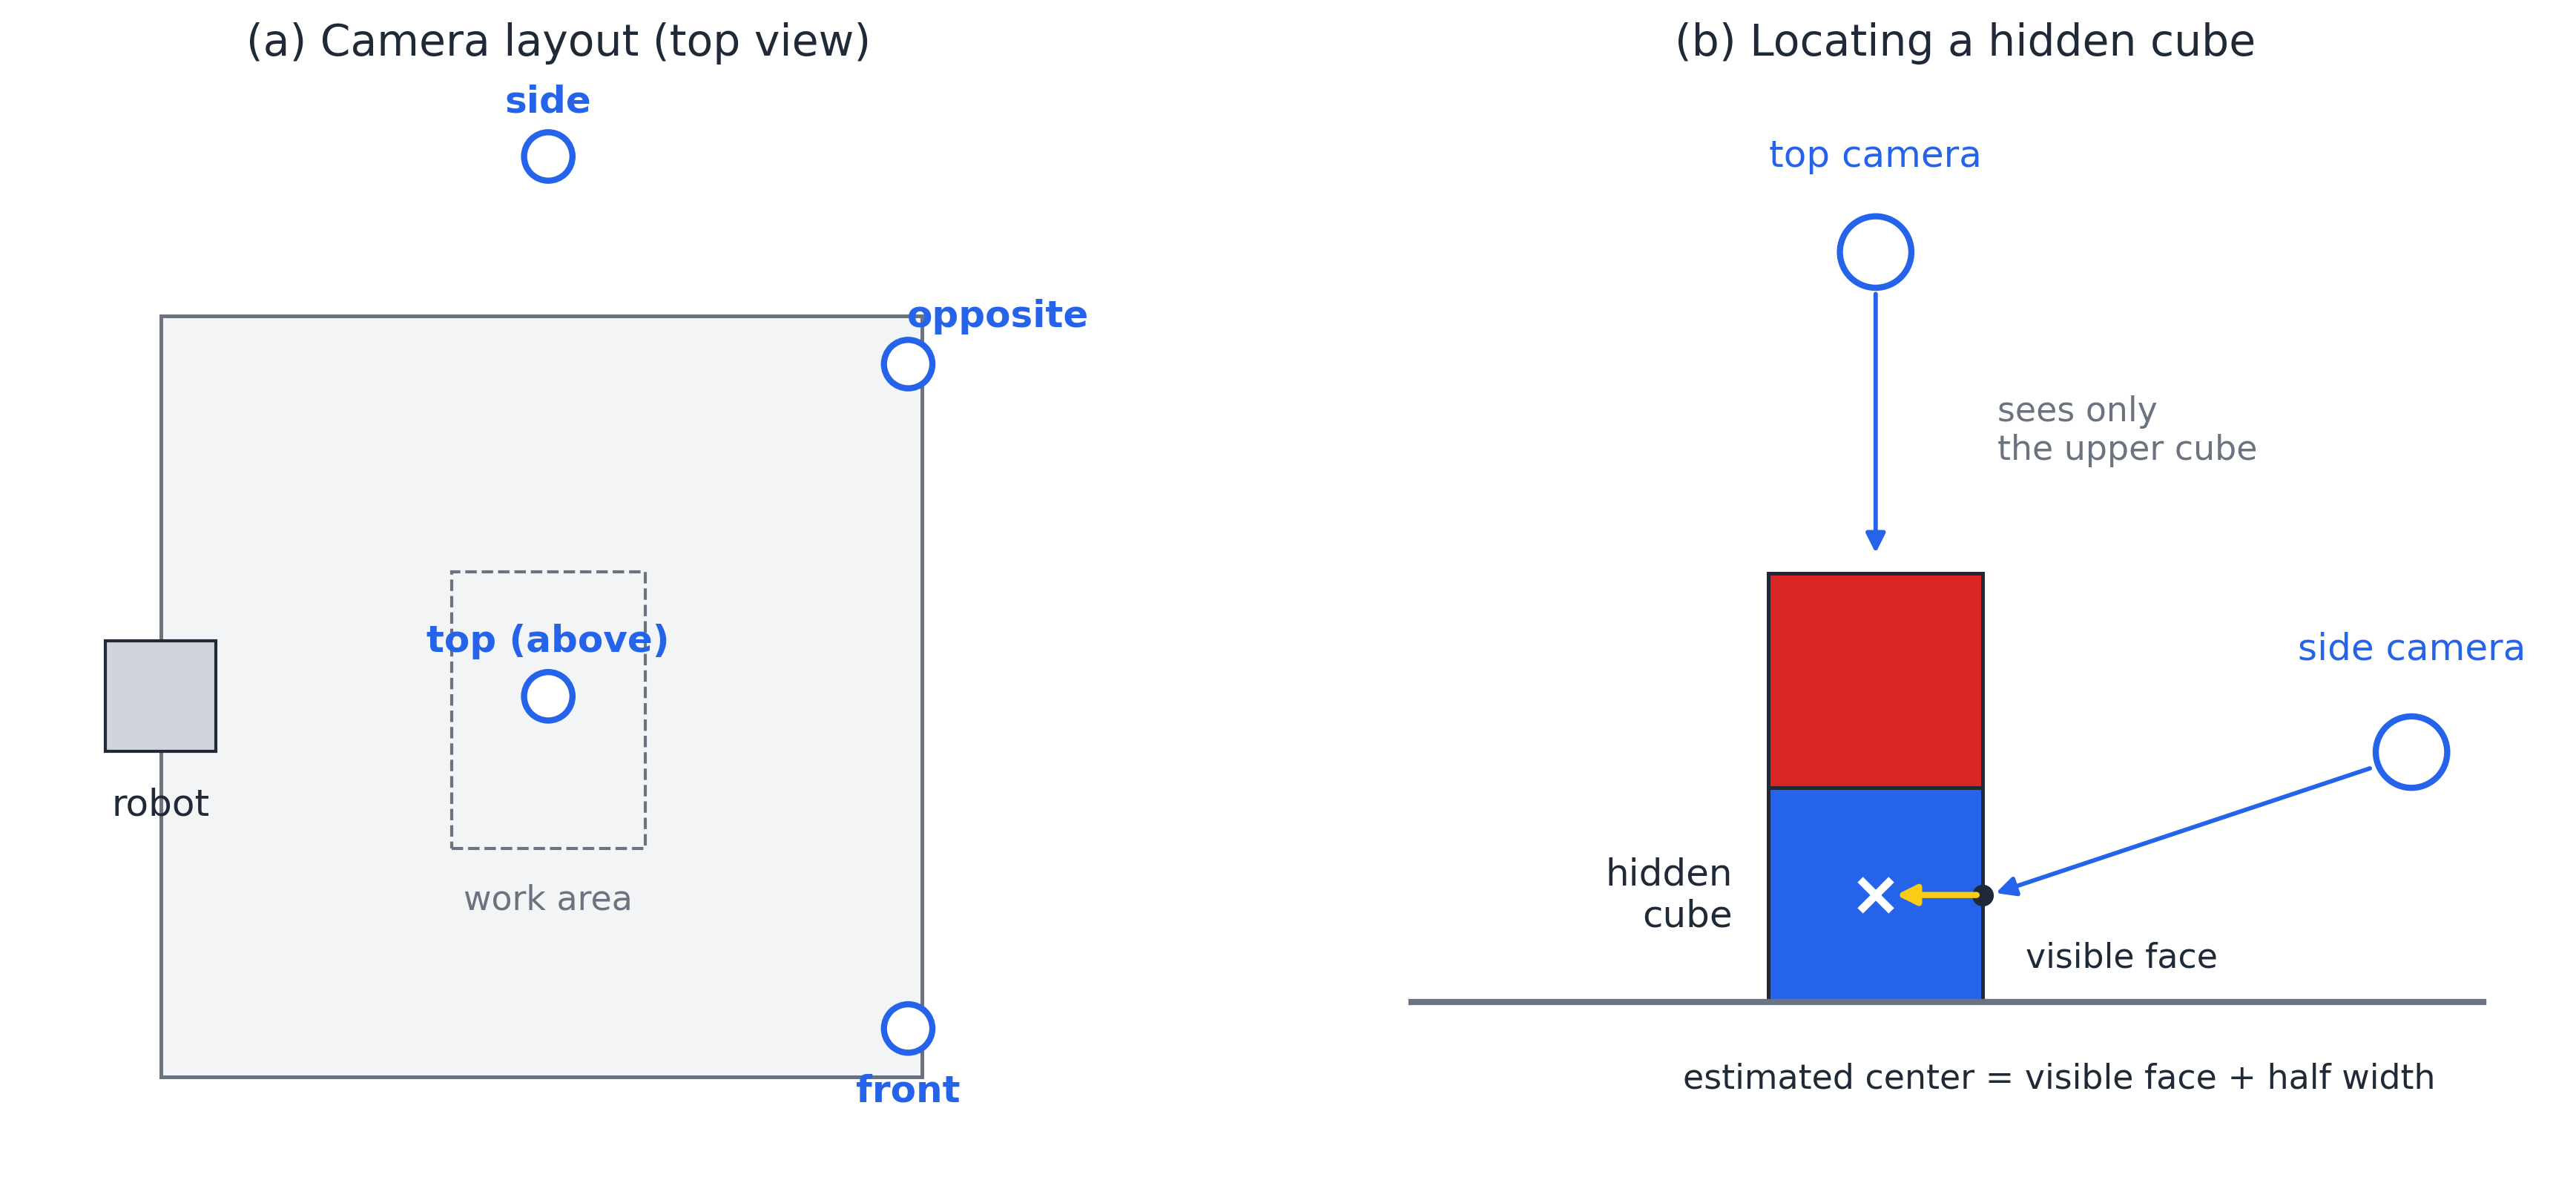
\includegraphics[width=\textwidth]{fig3_cameras.png}
\caption{(a) Placement of the cameras around the workspace. (b) Estimating the center of a covered cube from a side camera.}
\label{fig:cams}
\end{figure}

\subsection{Code Generation and Safe Execution}

The \texttt{gpt-6-luna} model was used for code generation. The model is given the measured object positions, the placement instruction for the task type, the current motion settings, and any correction rules from calibration. The model generates a straight-line Python program that uses only five commands: \texttt{get\_object\_position}, which reads the position of an object; \texttt{grasp}, which grasps and lifts a cube; \texttt{move\_to}, which moves the gripper to a given point; \texttt{release}, which releases the cube; and \texttt{home}, which returns the robot to its initial pose. Before execution, the program is checked on its abstract syntax tree (AST). Programs containing loops, conditionals, module imports, or calls to functions other than these five commands are rejected.

The motion settings consist of four values: the transit height at which horizontal moves are made, the height from which a cube is released onto another cube, the spacing between cubes in a row, and the offset used in diagonal placement. Their default values are 0.56~m, 0.075~m, 0.062~m, and 0.062~m, respectively.

When automatic safe lifting is enabled, the robot rises before every horizontal move longer than 35~mm to a height that keeps it above the tallest detected object. This height is computed with Eq.~\eqref{eq:safez}:
\begin{equation}
\begin{aligned}
z_{\text{safe}} = \max\Big(&z_{\text{transit}},\ \min\big(0.82,\ \max(0.47,\ z_{\text{top}}) + 0.11\big),\\
&\min\big(0.82,\ z_{\text{goal}} + 0.085\big)\Big)
\end{aligned}
\label{eq:safez}
\end{equation}
where $z_{\text{transit}}$ is the transit height in the motion settings, $z_{\text{top}}$ is the top surface of the tallest detected object, and $z_{\text{goal}}$ is the goal height of the move, all in meters.

Target joint angles are solved with inverse kinematics, and the robot is driven to them along a fifth-order minimum-jerk time profile~\cite{flash1985coordination}. Each joint is controlled at 240~Hz by the proportional-derivative (PD) controller in Eq.~\eqref{eq:pd}:
\begin{equation}
s(\tau) = 10\tau^3 - 15\tau^4 + 6\tau^5, \qquad \mathbf{u}(t) = K_p\left(\mathbf{q}_{\text{ref}}(t) - \mathbf{q}(t)\right) - K_d\,\dot{\mathbf{q}}(t)
\label{eq:pd}
\end{equation}
where $\tau \in [0, 1]$ is normalized time, $\mathbf{q}$ are the joint angles, $\mathbf{q}_{\text{ref}}$ is the reference trajectory, and $K_p$ and $K_d$ are the controller gains. The gripper grasps a cube with a force limit of 75~N, and the robot does not start a horizontal move until both fingers are verified to be in contact with the cube.

\subsection{Vision-Language Critic and Calibration}

At the end of each calibration iteration, a VLM critic decides whether the task succeeded. The \texttt{gpt-4.1} model was used as the critic. The critic is given images of the scene from the front, top, and side cameras together with the detected object positions, and is asked for a success decision and a failure type. When the critic's answer is ambiguous or not in the expected format, it is not counted as a success and is recorded as an evaluation error.

Six failure types were observed in preliminary trials. The failure types and the change that calibration makes for each are given in Table~\ref{tab:failures}. When an iteration fails, the motion settings of the corresponding task type are updated according to the values in the table, and a short correction rule for the failure type is saved. At most one rule is kept per failure type. Because records are kept per task type, the same record is used when the same task is requested with different words.

\begin{table}[htbp]
\centering
\caption{Failure types and the changes made by calibration.}
\label{tab:failures}
\begin{tabularx}{\textwidth}{@{}l Y Y@{}}
\toprule
Failure type & Description & Change made by calibration \\
\midrule
Order error & The cubes are stacked in the wrong order. & A rule is added not to touch the lower cube and to stack the cubes from the bottom up. \\
Alignment error & The cubes in a row or diagonal are at the wrong spacing. & The spacing between cubes is fixed at 62~mm. \\
Toppling & A cube released from too high bounced and toppled. & The release height is lowered from 0.075~m to 0.052~m. \\
Collision & The robot or the carried cube hit an obstacle or the tower. & The transit height is raised from 0.56~m to 0.68~m. \\
Box rim & The cubes were released at the same point in the box and spilled over the rim. & Three separate placement points inside the box are used. \\
Hidden cube & The lower cube could not be seen, or an old position was used. & Cube positions are measured again after every release. \\
\bottomrule
\end{tabularx}
\end{table}

\section{Experimental Setup and Results}

\subsection{Compared Methods and Evaluation}

RoboTeach was compared with four methods. The same model (\texttt{gpt-6-luna}) was used for code generation in all methods.
\begin{itemize}[leftmargin=*]
\item \textbf{Single camera:} The language model generates code using only object positions measured by the overhead camera. Task parsing, safe lifting, and calibration are not used.
\item \textbf{Four cameras:} Identical to the single-camera method, except that object positions are measured with four cameras. This method is Code-as-Policies~\cite{liang2023cap} run under the same perception conditions as RoboTeach and serves as the main baseline.
\item \textbf{Verbal correction:} In addition to the four-camera method, the correction suggestions written by the critic during calibration trials are saved and given to the language model in later trials. Suggestions are saved under the task name generated by the language model.
\item \textbf{Verbal correction (direct):} Identical to verbal correction, except that saved suggestions are added directly to the command of the corresponding task without matching task names.
\end{itemize}

Thirty different random initial scenes were used for each task, and all methods were tested on the same 180 scenes. Calibration iterations used scenes different from these. In the evaluation of RoboTeach, commands were worded differently from, but had the same meaning as, those used during calibration. To measure robustness, an additional experiment was run in a perturbed environment in which physics and sensor parameters were randomized. In this environment, cube mass was drawn from 0.084--0.156~kg, the cube friction coefficient from 1.2--2.8, and the table friction coefficient from 1.0--2.2; 3~mm noise was added to depth measurements, and the cameras were shifted by up to 3~mm and 1.5$^\circ$.

Success rates are reported with 95\% Wilson confidence intervals. Results of two methods on the same scenes were compared with the exact McNemar test. Confidence intervals of success differences were computed with a task-stratified bootstrap using 5,000 resamples. Differences are reported in percentage points (pp).

\subsection{Main Results}

Table~\ref{tab:main} shows the number of successful trials of each method on each task. Each cell gives how many of the 30 trials of that task succeeded. The last row gives the total over the six tasks and the overall success rate.

\begin{table}[htbp]
\centering
\caption{Successful trials per task for each method (30 trials per task).}
\label{tab:main}
\begin{tabularx}{\textwidth}{@{}l C C C C@{}}
\toprule
Task & Single camera & Four cameras & Verbal correction & RoboTeach \\
\midrule
Tower & 7 & 7 & 7 & 21 \\
Row & 3 & 9 & 7 & 28 \\
Diagonal & 13 & 26 & 23 & 25 \\
Box & 10 & 11 & 10 & 24 \\
Swap & 9 & 24 & 22 & 29 \\
Obstacle & 26 & 29 & 28 & 30 \\
\midrule
\textbf{Total (180)} & \textbf{68 (37.8\%)} & \textbf{106 (58.9\%)} & \textbf{97 (53.9\%)} & \textbf{157 (87.2\%)} \\
\bottomrule
\end{tabularx}
\end{table}

RoboTeach completed 157 of 180 trials and outperformed the four-camera method by 28.3~pp (95\% CI: 21.1--35.6~pp, $p < 0.001$). The largest differences occurred in the Row (28 vs.\ 9), Box (24 vs.\ 11), and Tower (21 vs.\ 7) tasks. In these tasks, the four-camera method mostly placed cubes at wrong spacings, released them at the same point in the box, or toppled them by releasing them from too high. In the Diagonal task, no clear difference was observed between the two methods (25 vs.\ 26). Moving from one camera to four cameras increased success mainly in the Diagonal (13 to 26) and Swap (9 to 24) tasks. In these two tasks, one of the cubes lies under another cube initially or during placement.

The verbal correction method was 5.0~pp behind the four-camera method (97 vs.\ 106, $p = 0.272$). For none of the six tasks was a suggestion saved during calibration found during evaluation, because the language model generated different names for the same task in two commands. When suggestions were given directly to the corresponding task, success dropped to 71/180 (39.4\%). This shows that correction suggestions given as plain text did not increase success on these tasks but reduced it.

In the perturbed environment, the success of RoboTeach dropped from 87.2\% to 81.7\% (147/180), and that of the four-camera method from 58.9\% to 54.4\% (98/180). The difference between the two methods remained at 27.2~pp in this environment ($p < 0.001$). The largest drop was observed in the Tower task, where a four-cube tower is built (21 to 15).

\begin{figure}[htbp]
\centering
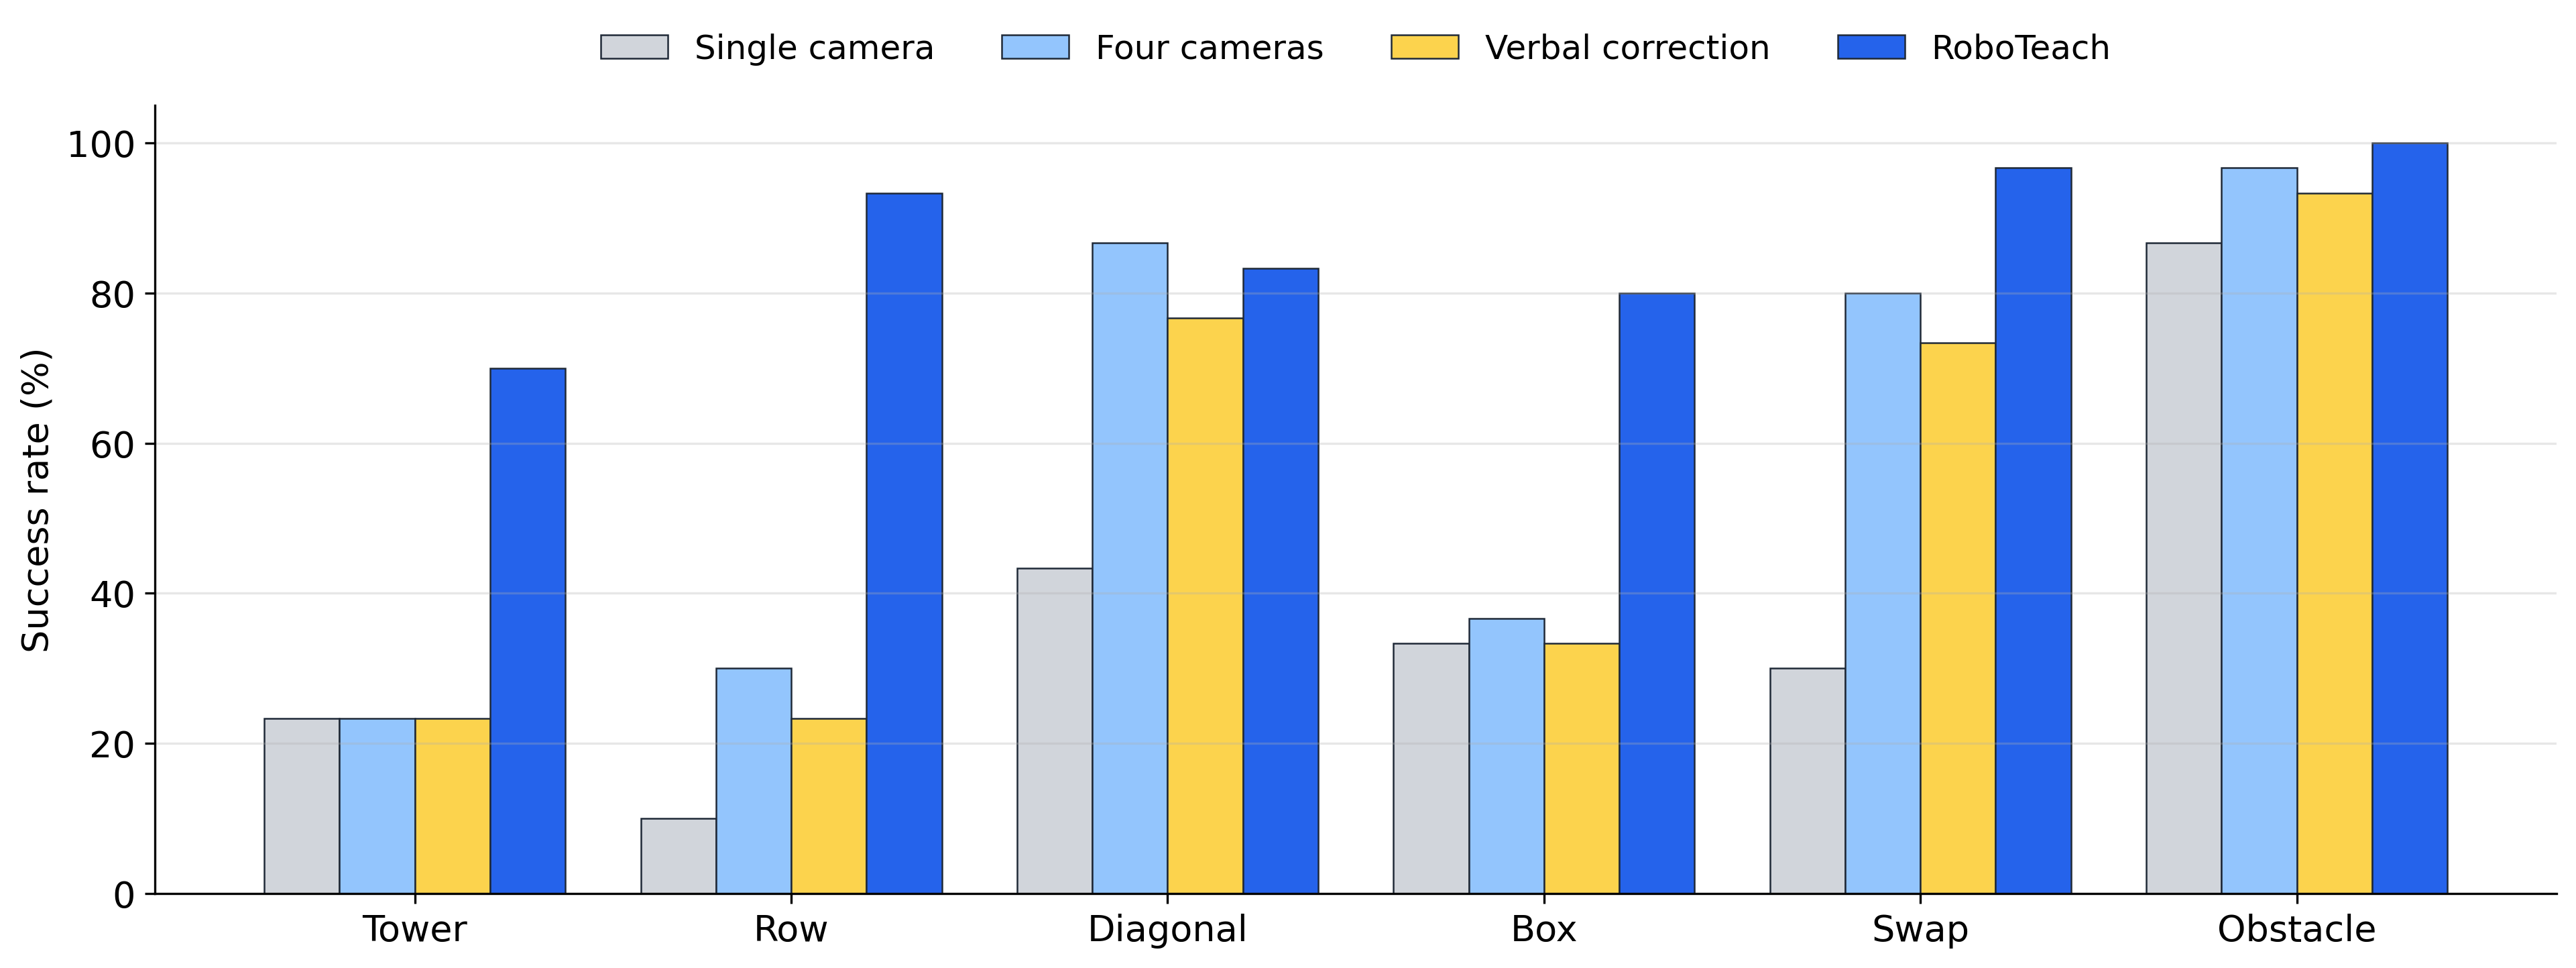
\includegraphics[width=\textwidth]{fig4_results.png}
\caption{Success rates of the methods per task.}
\label{fig:results}
\end{figure}

\subsection{Ablation Experiments}

To measure the contribution of each component, the components of RoboTeach were disabled one at a time and the system was tested again on the same 180 scenes. The results are given in Table~\ref{tab:ablation}. The difference column shows by how many percentage points success changed relative to the full system when the component was disabled.

\begin{table}[htbp]
\centering
\caption{Success when components are disabled one at a time (180 trials).}
\label{tab:ablation}
\begin{tabularx}{\textwidth}{@{}Y c c c@{}}
\toprule
Disabled component & Successful trials & Difference (pp) & $p$ \\
\midrule
None (full system) & 157 & -- & -- \\
Correction rules & 153 & $-2.2$ & 0.503 \\
Motion settings and safe lifting & 146 & $-6.1$ & 0.071 \\
Side cameras (overhead camera only) & 119 & $-21.1$ & $< 0.001$ \\
Task parsing & 71 & $-47.8$ & $< 0.001$ \\
\bottomrule
\end{tabularx}
\end{table}

The largest drop occurred when task parsing was disabled. In this case, the language model receives no placement instruction for the task type, and the Swap task is not split into sub-steps. Success dropped from 29 to 2 in the Swap task and to 5 in the Tower and Row tasks. Disabling the side cameras mainly affected the Row (28 to 10) and Diagonal (25 to 15) tasks. Resetting the motion settings to their defaults and disabling safe lifting did not change overall success significantly, but reduced success in the Obstacle task from 30 to 19 ($p < 0.001$). In this task, the robot does not pass over the wall at a sufficient height. Disabling the correction rules made no significant difference. Because motion settings and safe lifting were disabled together in this experiment, their contributions could not be measured separately. The contribution of calibration is therefore examined with separate experiments in Section~\ref{sec:calib}.

\subsection{Contribution of Calibration}
\label{sec:calib}

During calibration in the main experiment, the critic judged the first two iterations successful for four of the six task types (Tower, Row, Box, Obstacle), and the default settings were not changed. Settings were updated only for the Diagonal and Swap tasks. In both tasks, the transit height was set to 0.68~m, the release height to 0.052~m, and one rule was saved. In the Swap task, calibration reached the limit of five iterations because the critic rejected some iterations even though the simulator judged all five successful.

The effect of the calibration records was measured with two separate experiments. In the first experiment, task parsing, four cameras, and automatic safe lifting were kept enabled, and the two arms differed only in whether the calibration records (motion settings and correction rules) were used. Calibrated settings gave 154/180 (85.6\%) and default settings 159/180 (88.3\%), and the difference was not significant ($p = 0.332$). This indicates that safe lifting already removes the effect of a low transit height.

In the second experiment, automatic safe lifting was disabled and the calibration loop was run again for each task type under this condition. Calibration updated the settings for the Tower, Diagonal, and Swap tasks and left the defaults unchanged for the Row, Box, and Obstacle tasks. Default settings gave 144/180 (80.0\%) and calibrated settings 149/180 (82.8\%). Calibration increased success by 2.8~pp, but the difference was not significant (95\% CI: $-2.8$ to 8.3~pp, $p = 0.442$).

Two observations from this experiment are important. First, in the Obstacle task, 11 of 30 trials failed with the default settings, yet during calibration the critic judged the first two iterations successful and the settings were not changed. Calibration that stops after two consecutive successful iterations cannot catch the failure in tasks with such intermediate success rates. Second, in tasks whose settings did not change, success differences of up to four trials per task were observed although both arms ran with the same settings (for example, 24 vs.\ 28 in the Box task). These differences arise because the language model generates different code in each run. Small differences at the task level should therefore be interpreted with care.

\subsection{Perception and Command Parsing Accuracy}

Perception accuracy was evaluated by comparing positions measured in 60 scenes with the ground-truth positions in the simulator. In 30 of the scenes all cubes are visible, and in the other 30 one cube lies under another cube. Table~\ref{tab:perception} shows the position error of the single overhead camera and of the four cameras, together with the share of measurements whose error is below 40~mm. The error is given as root mean square error (RMSE) in millimeters. The 40~mm threshold represents the largest error acceptable for a successful grasp.

\begin{table}[htbp]
\centering
\caption{Position estimation error (RMSE, mm) and share of measurements with error below 40~mm.}
\label{tab:perception}
\begin{tabularx}{\textwidth}{@{}Y c c c c@{}}
\toprule
 & \multicolumn{2}{c}{Single camera} & \multicolumn{2}{c}{Four cameras} \\
\cmidrule(lr){2-3}\cmidrule(l){4-5}
Condition & RMSE & $<$40~mm & RMSE & $<$40~mm \\
\midrule
All objects visible & 23.9 & 83.3\% & 2.6 & 100\% \\
Covered cube & 43.9 & 73.3\% & 27.9 & 100\% \\
Depth noise, all objects & 24.1 & 83.3\% & 4.0 & 100\% \\
Depth noise, covered cube & 44.1 & 66.7\% & 27.7 & 100\% \\
Camera pose error, all objects & 28.5 & 83.3\% & 15.3 & 100\% \\
Camera pose error, covered cube & 47.2 & 50.0\% & 32.9 & 80.0\% \\
\bottomrule
\end{tabularx}

\vspace{2pt}
\begin{minipage}{\textwidth}\small
\textit{Note:} In the depth noise condition, noise with a standard deviation of 3~mm was added to depth measurements. In the camera pose error condition, images were rendered with the cameras shifted by 3~mm and 1.5$^\circ$, but the unshifted camera parameters were used for position computation.
\end{minipage}
\end{table}

The error of the single overhead camera increases for tall objects such as the box and the wall, because the camera sees their top edges instead of their centers. With all objects visible, the error of the four cameras is 2.6~mm. For a covered cube the error rises to 27.9~mm, but all measurements remain below the 40~mm threshold. With wrong camera poses, this share drops to 80\% for covered cubes. The four-camera error also remained low for objects other than cubes: 4.6~mm for a cylinder with a diameter of 48~mm and 4.7~mm for a prism 96~mm long, and both objects were grasped in all 30 trials at 30 different orientations.

Command parsing accuracy was measured with 180 different command phrasings, 15 Turkish and 15 English for each task. The parser correctly extracted the task type, object order, cube pairs, target box, and initially stacked cubes for all 180 phrasings. A simple matcher that looks only at keywords, ignoring sentence structure and initial state, gave correct results for 76 phrasings (42.2\%). When the language model was asked to generate a free task name for each command, it generated the same name for only 2 of 60 pairs of commands with the same meaning. This explains why the verbal correction method in Section~4.2 could not find its saved suggestions.

\subsection{Accuracy of the Vision-Language Critics}

The reliability of critic decisions was measured by comparing the decisions of two different critic models with ground-truth outcomes read from the simulator in 120 trials, of which 73 were successful and 47 failed. The compared models are \texttt{gpt-4.1}, which was used in calibration, and \texttt{gpt-6-luna}, which was used for code generation. In Table~\ref{tab:critic}, a ``false approval'' means that the critic counted a failed trial as successful, and a ``false rejection'' means that it counted a successful trial as failed. False approval is the most harmful error for calibration, because the faulty settings remain unchanged.

\begin{table}[htbp]
\centering
\caption{Critic decisions compared with simulator outcomes (120 trials).}
\label{tab:critic}
\begin{tabular}{@{}l c c@{}}
\toprule
 & \texttt{gpt-4.1} & \texttt{gpt-6-luna} \\
\midrule
Correct approval & 58 & 55 \\
Correct rejection & 39 & 45 \\
False approval & 8 & 2 \\
False rejection & 15 & 18 \\
Accuracy & 80.8\% & 83.3\% \\
Cohen's kappa & 0.61 & 0.67 \\
Median decision time & 1.6~s & 3.4~s \\
\bottomrule
\end{tabular}
\end{table}

According to the Landis and Koch classification, the kappa values of both critics fall in the ``substantial agreement'' band~\cite{landis1977kappa}. \texttt{gpt-6-luna} reduced the rate of approving failed trials from 17.0\% (8/47) to 4.3\% (2/47), but took about twice as long to decide. In an independently repeated second audit (72 successful and 48 failed trials), no significant difference was found between the accuracies of the two critics (78.3\% vs.\ 80.8\%, $p = 0.736$); however, \texttt{gpt-4.1} approved 13 failed trials and \texttt{gpt-6-luna} approved 3, and this difference in false approvals was significant ($p = 0.002$).

\section{Discussion and Limitations}

The results show that most of the success of RoboTeach comes from two components. The first is task parsing. The task-specific placement instructions that the parser gives the language model are the largest source of the gain over the four-camera method. These instructions were written by hand for each task type, which means that extending the system to a new task type also requires writing an instruction for it. The second is multi-camera perception. The side cameras reduce position error mainly in tasks with covered cubes.

The contribution of calibration remained limited. With safe lifting enabled, calibration gave no additional gain; with safe lifting disabled, it updated the settings in the expected direction, but the increase in success did not reach significance. There are two reasons for this. First, the default settings and safe lifting are already sufficient for most tasks. Second, the stopping criterion of two consecutive successful iterations cannot catch failures that appear in only some trials of a task. A stopping criterion that uses more iterations or measures the success rate over several trials could reduce this limitation.

The study has further limitations. First, all experiments were run in PyBullet simulation, and the system was not tested on a real robot. A real setting includes effects absent from simulation, such as sensor noise, lighting changes, camera calibration errors, and finger compliance. Transfer to a real Franka Emika Panda would require replacing color-threshold segmentation with a method based on vision-language features~\cite{radford2021clip}, calibrating the cameras to the robot, and validating each task with at least 30 trials. Second, in the Obstacle task, collisions between the robot and the wall are not checked; only the final state is evaluated. Third, the parser recognizes only Turkish and English commands. Although the language model used for code generation can understand other languages, commands in those languages cannot be assigned to the correct task type. Fourth, \texttt{gpt-4.1} and \texttt{gpt-6-luna} differ both in model family and in reasoning capability, so it cannot be determined which of these two factors causes the difference in Table~\ref{tab:critic}. Fifth, the perception method is designed for regular shapes such as cubes, cylinders, and prisms. Irregularly shaped objects would require shape completion methods.

\section{Conclusion}

This paper presented RoboTeach, a training-free system that converts natural language commands into robot motion. In simulation, the system outperformed an open-loop baseline using four cameras by 28.3~pp on six tabletop tasks. Most of the gain comes from task parsing and multi-camera perception. The calibration loop gave no additional gain while safe lifting was enabled and increased success by a non-significant margin while it was disabled. The findings are limited to the six task types and the simulation conditions tested.

\section*{Data and Code Availability}

The simulation environment, the perception, task parsing, code generation, and calibration modules, the experiment scripts, and all result files are openly available at \url{https://github.com/Mahmut-OZTURK/robotech}. The random scene indices and model settings used in the experiments are included in the experiment scripts in the repository.

\section*{Declarations}

\textbf{Funding:} This research did not receive any specific grant from funding agencies in the public, commercial, or not-for-profit sectors.

\textbf{Declaration of competing interest:} The authors declare that they have no known competing financial interests or personal relationships that could have appeared to influence the work reported in this paper.

\textbf{CRediT authorship contribution statement:} [To be completed by the authors.]

\textbf{Declaration of generative AI use:} [To be completed by the authors.]

\bibliographystyle{elsarticle-num}
\bibliography{references}

\end{document}
